%
% Documento: Introdução
%

\chapter{Introdução}\label{chap:introducao}  

Define-se mobilidade como aquilo que tem “facilidade de se movimentar, andar, dançar.” \cite{mobilidade}, característica do que é móvel ou obedece às leis do movimento. 

Mobilidade Urbana já é um termo que não encontramos no dicionário, porém, de fácil compreensão, %quando analisamos às duas palavras juntas,
pois, logo relacionamos a algo que de fato é ou se assemelha, basicamente a condição
de se deslocar dentro de uma cidade, “campus”, bairro. %com objetivo de criarmos relações sociais, — como ir ao supermercado —, ou relações econômicas — como ir ao trabalho —, utilizando meios de transporte como carros, ônibus, metrô, etc.



No Brasil, com a Política Nacional de Mobilidade Urbana -- PNMU, aprovada em 2012, obriga estados e municípios com mais de 20 mil habitantes a terem um planejamento de expansão pensando em como as pessoas vão se locomover, considerando o crescimento urbano e populacional  \cite{lei12587}.

Segundo informe do Instituto de Pesquisa Econômica Aplicada -- IPEA, o aumento da produção automotiva no Brasil estimulou a crescente utilização de carros e motos em todo o território nacional. O fácil acesso a esses automóveis provocaram a redução da importância do transporte público na matriz modal, aumentou o tráfego e a emissão de poluentes \cite{ipea}.
 
As Cidades Inteligentes -- CI, hoje são vistas como uma das soluções para alguns problemas urbanos. As CI buscam sempre melhorar o estilo de vida dos cidadãos, ao administrar recursos, analisar a qualidade do ar, gerenciar resíduos, controlar o trânsito, entre outros \cite{chourabi}.

De acordo com \citeonline{namepardo}, o conceito de CI não chega a ser uma novidade no mundo acadêmico. O tema é amplamente discutido e ganhou uma nova dimensão quando passou a implementar Tecnologias da Informação e Comunicação -- TIC para construir infraestruturas e serviços de uma cidade.	

Tecnologias como GPS e \textit{Smartphones} são tendências no atual momento das CI. Estes dispositivos propiciam a criação de novas soluções inteligentes. Com o recurso do GPS, a capacidade de localizar ou buscar endereços nos mapas digitais facilita bastante ao traçar uma rota, meio este que é utilizado por serviços como Google Maps\footnote{Disponível em: https://www.google.com.br/maps. Acesso em: 20 Jun. 2020.}.

Portanto, com o fim de amenizar o impacto dos combustíveis fósseis e facilitar o trajeto das pessoas, a  Mobilidade inteligente que é um dos conceitos de CI, utiliza recursos tecnológicos para resolver problemas relacionados a Mobilidade Urbana.

Mobilidade Inteligente envolve acessibilidade, praticidade, soluções modernas e sustentáveis com forte suporte tecnológico para facilitar os deslocamentos, especialmente para usuários de transporte coletivo e privado.

\section {Problema}
\begin{comment}
	Na cidade de Macapá e Santana, as duas maiores cidade do Amapá, o número de transporte coletivo é baixo,
	existe apenas duas rodovias que interligam as cidades, 
	se locomover se torna difícil \cite{sau2018}. % 
	
	Com tantos problemas aparentes causadas pelo grande inchaço populacional que  vive nas áreas urbanas, cerca de 80\% da população das duas cidades reside em áreas urbanas e sofre com a insuficiência do sistema de transporte público oferecido \cite{tostes}.
\end{comment}

Os acadêmicos da Universidade Federal do Amapá - Unifap têm como transporte público os ônibus e táxis, e no caso da cidade de Santana, os alunos têm apenas uma linha de ônibus que faz a rota intermunicipal \cite{sau2018}.

No período de 2010 a 2017, a cidade de Macapá teve um aumento total de 13 ônibus ativos, e nesse mesmo período houve um aumento de 57 967 pessoas que utilizam o transporte coletivo diariamente \cite{sau2018}. %dados da Companhia de Trânsito do Amapá -- CTMAC \footnote{text}. 
 
Cabe ressaltar que muitas rotas não assistem todas as áreas da cidade sendo necessário trocar de ônibus ou meio de transporte, o que aumenta o tempo de uso do coletivo para chegar ou sair da universidade. \cite{galiano}.

\citeonline{sau2018} afirma que Macapá não possui outras opções de transporte coletivo além de ônibus, táxis e mototáxis, apenas lotações (corridas ilegais) e aplicativos de transporte de passageiros.

Questões relacionadas a Mobilidade Urbana foi levantado no trabalho, como ``Quais os principais problemas enfrentados com o transporte que utiliza?'' ou ``Você se sente satisfeito com o transporte que utiliza?'', estás perguntas serão respondidas ao decorrer da pesquisa.






\section{Justificativa}



Considerando o que já foi apresentado como problema sobre a Mobilidade da cidade de Macapá e Santana, o trabalho buscou uma solução existente que pudesse ser alcançada em aspectos financeiros tanto para a Unifap quanto para os alunos. 

Está solução de Mobilidade Inteligente não só busca ser uma alternativa entre ônibus, táxis, mototáxis, ser mais prático e consumir menos tempo no trajeto, mas também tem como iniciativa nossa incluir o espirito colaborativo entre os integrantes da comunidade por intermédio da oferta de carona.

\mnote{Argumentar mais na justificativa, falar mais sobre a solução que escolhemos, além de aspectos financeiros, podemos dizer que escolhemos essa soluçãi entre as outras vistas porque nela é possível alterar o código, alterar informações no app conforme nossa demanada e necessidade e nela podemos restringir os usuários que acessam. 
Acrescentar a importancia da mobilidade inteligente nas soluções de problemas urbanos,
}


\begin{comment}
que os problemas de mobilidade existentes
atualmente em Macapá atingem diretamente a comunidade acadêmica da Universidade Federal do Amapá, este trabalho buscará entender o perfil e as principais dificuldades da comunidade acadêmica, e, a partir de um estudo de soluções existentes no contexto de CI para propor uma solução que seja viável e admissível para a comunidade acadêmica da Unifap

%E para somar
%Além disso, os altos índices de criminalidade 
%afligem a população que precisa do transporte coletivo, principalmente à noite em paradas escuras
%, realidade da parada que se localiza em frente à Universidade. Muitos alunos sofrem da falta de ônibus ou de apenas uma empresa cobrir a área onde o estudante mora, e ainda existe na cidade muitas áreas sem uma empresa de ônibus cobrindo a área.  [foto ou materia que fale dessa situação]
%	\mnote{Patrícia: infelizmente não temos como afirmar isso sem uma referência e dados concretos. Melhor retirar esse parágrafo.}
%
\end{comment}

\section {Objetivos}

O projeto teve como principal foco a implementação de uma solução de mobilidade inteligente para a universidade, além de elaborar questionários que foram respondidos por integrantes da comunidade acadêmica com fins para o próprio entendimento do trabalho. 

\subsection{Objetivo Geral}
Este trabalho teve como objetivo implementar uma solução de mobilidade inteligente existente que sirva como alternativa de entrada e saída dos acadêmicos da Unifap -- Campus Macapá.

\begin{comment}
Este trabalho tem como objetivo principal o estudo sobre Mobilidade Inteligente
considerando o contexto de mobilidade relacionado à Universidade Federal do Amapá
e realizar o debate sobre a viabilidade de utilização pela comunidade acadêmica em geral (docentes, discentes e técnicos) de soluções tecnológicas existentes, visando oferecer alternativa(s) de transporte que dê acesso e diminua problemas diários enfrentados para chegar e/ou sair da universidade.
\end{comment}

\subsection{Objetivos Específicos}

Para alcançar o objetivo geral, definimos os seguintes objetivos específicos:

\begin{enumerate}
%\item Estudo sobre Cidades Inteligente focado em Mobilidade Inteligente;

\item Identificar o perfil da comunidade acadêmica da Unifap por meio do questionário; \mnote{Como assim perfil? Argumente mais sobre..}


\item Realizar um levantamento de soluções de Mobilidade Inteligente;

%\item Análise comparativa dos diferentes tipos de soluções de Mobilidade Inteligente 
%considerando o perfil da comunidade acadêmica da Unifap;

\item Definir os requisitos da solução mais viável para a comunidade acadêmica da Unifap;

%\item Definir a proposta de projeto de solução de Mobilidade Inteligente considerando o perfil da comunidade acadêmica da Unifap;

%\item Levantamento das soluções disponíveis que se encaixam dentro dos requisitos;

%\item Triagem das soluções encontradas;

\item Aplicar a solução de mobilidade em ambiente de produção; \mnote{Ambiente de produção, ou na internet; ambiente de testes para terceiros}

\item Avaliar a solução de mobilidade por intermédio de um questionário aplicado à comunidade;

\end{enumerate}

\begin{comment}


\begin{enumerate}
\item \textit{Realizar um questionário.}
\item \textit{Analisar os resultados do questionário.}
\item \textit{Preparar o ambiente de desenvolvimento.}
\item \textit{Estudar as ferramentas que serão utilizadas no projeto.}
\item \textit{Procurar soluções similares com o objetivo de tirar ideias utéis para o projeto.}
\item \textit{Verificar soluções que já existem com a mesma proposta de caronas solidárias, reutilizar código se for de código aberto.}
\item \textit{Integrar os serviços de gestão acadêmica com a ferramenta que irá ser criada/reutilizada na proposta.}


\end{enumerate}
\end{comment}




%Na Figura \ref{bigdata}, temos:

%\begin{figure}[!hbtp]
%	\centering
%	\caption{Perspectivas de \textit{big data}.}
%	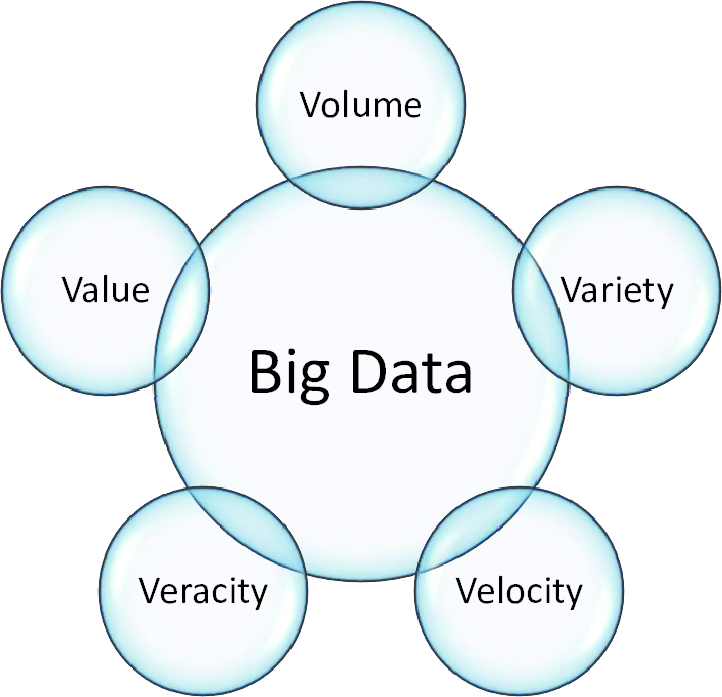
\includegraphics[scale=.75]{./04-figuras/bigdata.png}
%	\label{bigdata}
%	\fonte{\cite{elragal:2014}}
%\end{figure}



%\section {Exemplo de Seção}

%\subsection{Exemplo de Subseção}

%\subsubsection{Exemplo de Subseção da Subseção}

%\section {Tabela}
%Na Tabela \ref{tabela}, temos: 

%\begin{table*}[ht]
%	\centering
%	\caption{Exemplo de Tabela.}
%	\label{tabela}
%	\begin{tabular}    %{p{0.49\linewidth}p{0.03\linewidth}p{0.03\linewidth}p{0.03\%linewidth}p{0.03\linewidth}p{0.21\linewidth}}
%		\hline
%		Ítem & Ítem & Ítem & Ítem & Ítem & Ítem\\
%		\hline
%		Ítem & Ítem & Ítem & Ítem & Ítem & Ítem\\
%		\hline
%	\end{tabular}
%\end{table*}